\documentclass[12pt,a4paper]{ctexart}

% =========================
% 基础宏包
% =========================
\usepackage{amsmath,amssymb}
\usepackage{graphicx}
\usepackage{float}
\usepackage{booktabs}
\usepackage{array}
\usepackage{tabularx}
\usepackage{listings}
\usepackage[hidelinks]{hyperref}
\usepackage{geometry}
\usepackage{setspace}
\usepackage{tocloft}
\usepackage{fancyhdr}
\usepackage{xcolor}
\usepackage{subcaption}
\usepackage{caption}
\usepackage{enumitem}

% =========================
% 页面设置
% 参考期末报告的紧凑风格
% =========================
\geometry{
    left=2.25cm,
    right=2.25cm,
    top=2.15cm,
    bottom=2.15cm
}

\setstretch{1.05}

\setlist[itemize]{
    leftmargin=2em,
    itemsep=0.08em,
    topsep=0.12em
}

\setlist[enumerate]{
    leftmargin=2em,
    itemsep=0.08em,
    topsep=0.12em
}

\captionsetup{
    font=small,
    labelfont=bf
}

\renewcommand{\arraystretch}{1.12}
\setlength{\tabcolsep}{4.5pt}
\emergencystretch=2em

% =========================
% 页眉页脚
% =========================
\pagestyle{fancy}
\fancyhf{}

\fancyhead[L]{编译系统原理}
\fancyhead[R]{谭锦睿 2412771 \quad 王帅 2413995}

\fancyfoot[C]{\thepage}

\setlength{\headheight}{15pt}
\renewcommand{\headrulewidth}{0.4pt}
\renewcommand{\footrulewidth}{0pt}

% =========================
% 目录与标题格式
% =========================
\setlength{\cftbeforesecskip}{0.28em}

\ctexset{
    section/format=\raggedright\bfseries\large,
    subsection/format=\raggedright\bfseries\normalsize,
    subsubsection/format=\raggedright\bfseries\normalsize
}

% =========================
% 代码格式
% 只展示必要命令或关键片段
% =========================
\definecolor{codebg}{gray}{0.95}

\lstdefinestyle{plaincode}{
    basicstyle=\ttfamily\small,
    breaklines=true,
    frame=none,
    numbers=none,
    showstringspaces=false,
    keywordstyle=\bfseries,
    commentstyle=\itshape,
    stringstyle=\ttfamily,
    backgroundcolor=\color{codebg},
    tabsize=2,
    columns=fullflexible
}

\lstset{style=plaincode}

% =========================
% 王帅部分临时占位
% 最终提交前删除提示框
% =========================
\newcommand{\wsplaceholder}[1]{%
\begin{center}
\fbox{%
\begin{minipage}{0.92\textwidth}
\small
\textit{王帅补充：#1}
\end{minipage}}
\end{center}
}

% =========================
% 标题信息
% =========================
\title{
\textbf{
编译系统原理预备工作实验报告\\[0.35em]
了解你的编译器：编译流程与目标代码实现
}
}

\author{
谭锦睿（2412771）
\quad
王帅（2413995）
}

\date{}

\begin{document}

\maketitle
\thispagestyle{empty}

\tableofcontents
\newpage

% =========================
% 摘要
% =========================
\begin{abstract}

本实验围绕编译器从高级语言源程序到目标程序的处理过程展开。首先以循环实现的阶乘 C 程序为例，利用 GCC 和 Clang/LLVM 观察预处理、词法分析、抽象语法树、LLVM IR、汇编、目标文件和链接等阶段的输出，并比较不同优化级别对生成代码的影响。在此基础上，设计了一段覆盖常量、数组、算术运算、条件分支、循环、函数调用和运行时输入输出的 SysY 程序，分别进行 LLVM IR 和 RISC-V 目标表示实现。RISC-V 部分进一步与 SysY 运行时库进行静态链接，并通过 QEMU 对普通输入和边界输入进行验证。进阶部分结合 AscendNPU IR 的 VecAdd 示例，对 MLIR 多层 Dialect 与渐进式 lowering 的基本思想进行了文档调研和分析。通过上述实验，加深了对编译器前端、中间表示、目标代码和运行时环境之间关系的理解。

\end{abstract}

\noindent
\textbf{关键词：}
编译器；LLVM IR；SysY；RISC-V；MLIR

% =========================================================
\section{实验任务与小组分工}
% =========================================================

\subsection{实验任务}

本次预备工作围绕“了解编译器”展开，目标并不是只完成一次程序编译，而是通过实际工具观察高级语言程序在编译过程中经历的不同表示形式，并理解这些表示之间的关系。

基础部分首先选择一个规模适中的 C 程序，利用 GCC 和 Clang/LLVM 提供的命令行选项，依次观察预处理结果、词法单元、抽象语法树、LLVM IR、汇编程序、目标文件和最终可执行文件。通过这些中间产物，可以将课堂中的编译流程具体落实到实际文件和指令中。

在此基础上，进一步设计具有代表性的 SysY 程序，使其覆盖数值运算、赋值、条件分支、循环、函数调用以及数组等语言结构，并分别手工实现等价 LLVM IR 和 RISC-V 汇编代码。实现后与课程提供的 SysY 运行时库进行链接，通过实际执行验证不同低层表示是否保持与源程序一致的语义。

进阶部分结合 AscendNPU IR 的 VecAdd 示例，对 MLIR 的 Dialect、多层中间表示以及渐进式 lowering 思想进行调研，从而将实验范围由传统通用编译器扩展到面向 AI 加速器的编译流程。

实验主要在 Windows + WSL2 Ubuntu 环境下完成。第一部分使用 GCC 13.3.0 和 LLVM 18；RISC-V 部分使用 GCC 15.1.0、GNU Binutils 2.45 和 qemu-riscv64 8.2.2。

\subsection{小组分工}

第一部分由两位成员共同完成，包括实验程序设计、编译流程命令执行、中间结果观察以及优化前后代码比较。第二部分以同一 SysY 测试程序作为语义基准，在保证最终输入输出一致的基础上分别完成 LLVM IR 和 RISC-V 两种实现。

\begin{table}[H]
\centering
\caption{小组成员分工}
\begin{tabularx}{\textwidth}{@{}p{2.4cm}p{2.2cm}X@{}}
\toprule
姓名 & 学号 & 主要工作 \\
\midrule

谭锦睿 &
2412771 &
负责 RISC-V 汇编实现，包括栈帧设计、数组地址计算、条件与循环控制流翻译、32 位整数运算、函数调用、SysY RISC-V 运行时库链接及 QEMU 执行验证；参与第一部分实验和进阶内容整理。 \\

王帅 &
2413995 &
负责 SysY 程序的 LLVM IR 手工实现，包括基本块组织、数组寻址、控制流翻译、运行时函数声明与链接以及执行验证；与谭锦睿共同完成第一部分实验。 \\

\bottomrule
\end{tabularx}
\end{table}

% =========================================================
\section{C 程序编译流程观察}
% =========================================================

\subsection{实验程序与总体流程}

实验选取循环实现的阶乘程序作为贯穿各阶段的示例。程序定义 \texttt{factorial(int n)} 函数，通过循环不断更新累乘结果，主函数读取整数后调用该函数并输出结果。该程序虽然规模较小，但同时包含函数定义、局部变量、循环、整数运算以及标准库函数调用，能够较完整地观察编译过程中不同阶段的变化。

输入 5 时程序输出 120，说明后续观察到的各类中间结果均对应一个功能正确的源程序。

\begin{figure}[H]
\centering
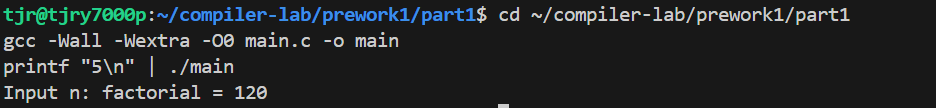
\includegraphics[width=0.76\textwidth]
{images/part1/part1_source_run.png}
\caption{阶乘程序运行结果}
\label{fig:source-run}
\end{figure}

整个处理过程可以概括为：

\[
\text{main.c}
\rightarrow
\text{main.i}
\rightarrow
\text{Token / AST}
\rightarrow
\text{LLVM IR}
\rightarrow
\text{Assembly}
\rightarrow
\text{Object}
\rightarrow
\text{Executable}.
\]

这些阶段并不是简单的文件格式变化，而是在不断降低程序的抽象层次。源程序强调程序员能够理解的语义结构，AST 强调语法关系，LLVM IR 开始显式体现基本块和数据访问，汇编程序则已经直接面向具体目标体系结构。

\subsection{预处理、词法与语法结构}

首先使用 GCC 的预处理选项：

\begin{lstlisting}
gcc -E main.c -o main.i
\end{lstlisting}

源文件 \texttt{main.c} 只有 33 行，而生成的 \texttt{main.i} 达到 847 行。主要原因是 \texttt{stdio.h} 等标准头文件中的声明被展开，同时源程序中定义的宏 \texttt{START\_VALUE} 已经被替换为常量 1。

\begin{figure}[H]
\centering
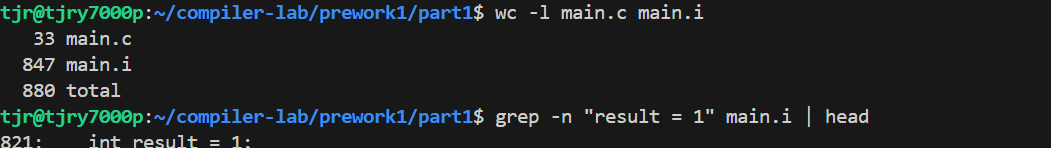
\includegraphics[width=0.72\textwidth]
{images/part1/part1_preprocess.png}
\caption{预处理前后的文件规模及宏展开结果}
\label{fig:preprocess}
\end{figure}

因此，预处理阶段仍属于源语言层面的处理。它不会直接生成机器代码，而是完成宏替换、头文件展开等工作，为后续真正的编译阶段准备完整输入。

进一步使用 Clang 输出 Token 和 AST。Token 输出中可以看到 \texttt{int}、\texttt{while} 等关键字，\texttt{factorial}、\texttt{result} 等标识符，以及括号、运算符和数值常量。AST 则进一步将这些线性的词法单元组织为树形语法结构。例如，\texttt{factorial} 对应 \texttt{FunctionDecl} 节点，循环对应 \texttt{WhileStmt}，表达式中的乘法和加法则对应 \texttt{BinaryOperator}。

\begin{figure}[H]
\centering

\begin{subfigure}[t]{0.48\textwidth}
\centering
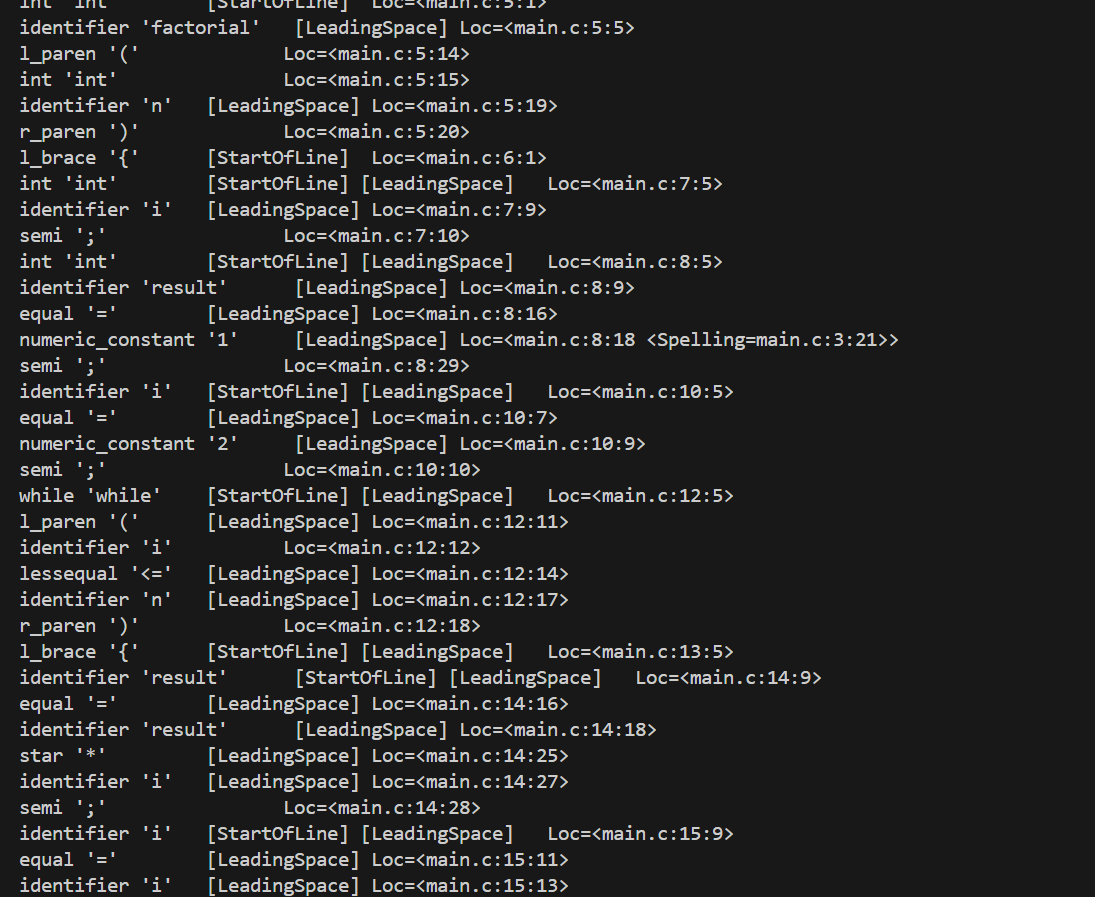
\includegraphics[width=\textwidth]
{images/part1/part1_tokens.png}
\caption{Token 输出}
\end{subfigure}
\hfill
\begin{subfigure}[t]{0.48\textwidth}
\centering
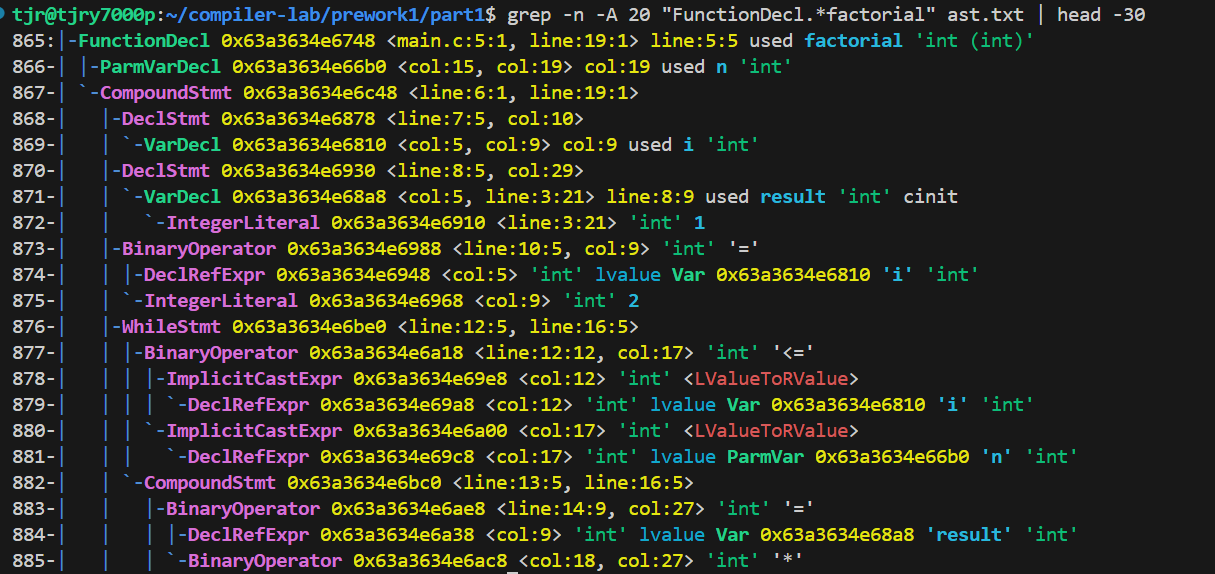
\includegraphics[width=\textwidth]
{images/part1/part1_ast.png}
\caption{AST 片段}
\end{subfigure}

\caption{词法单元与抽象语法树}
\label{fig:token-ast}
\end{figure}

这一过程体现了词法分析和语法分析的区别：前者回答“源程序由哪些词法单元组成”，后者进一步回答“这些词法单元按照什么语法结构组合”。

\subsection{LLVM IR、汇编与链接}

使用

\begin{lstlisting}
clang -S -emit-llvm -O0 main.c -o main.ll
\end{lstlisting}

生成 LLVM IR 后，可以观察到源程序中的局部变量通过 \texttt{alloca} 分配空间，通过 \texttt{load} 和 \texttt{store} 进行读写；循环条件使用 \texttt{icmp} 完成判断，并由 \texttt{br} 在不同基本块之间转移；乘法和循环变量递增则分别使用 \texttt{mul} 和 \texttt{add}。

\begin{figure}[H]
\centering

\begin{subfigure}[t]{0.48\textwidth}
\centering
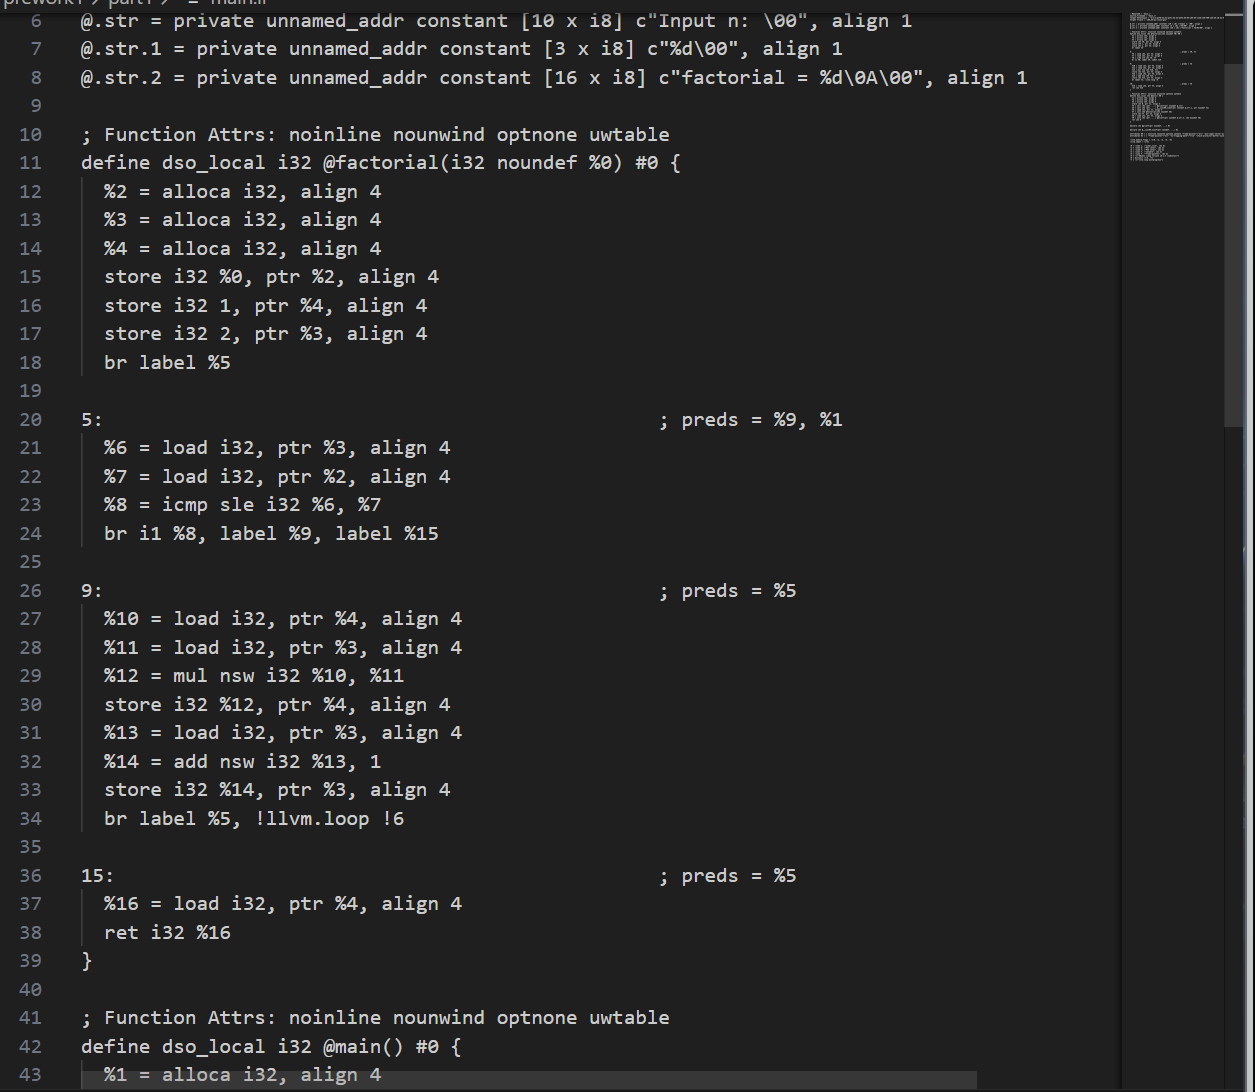
\includegraphics[width=\textwidth]
{images/part1/part1_llvm_ir.png}
\caption{LLVM IR}
\end{subfigure}
\hfill
\begin{subfigure}[t]{0.48\textwidth}
\centering
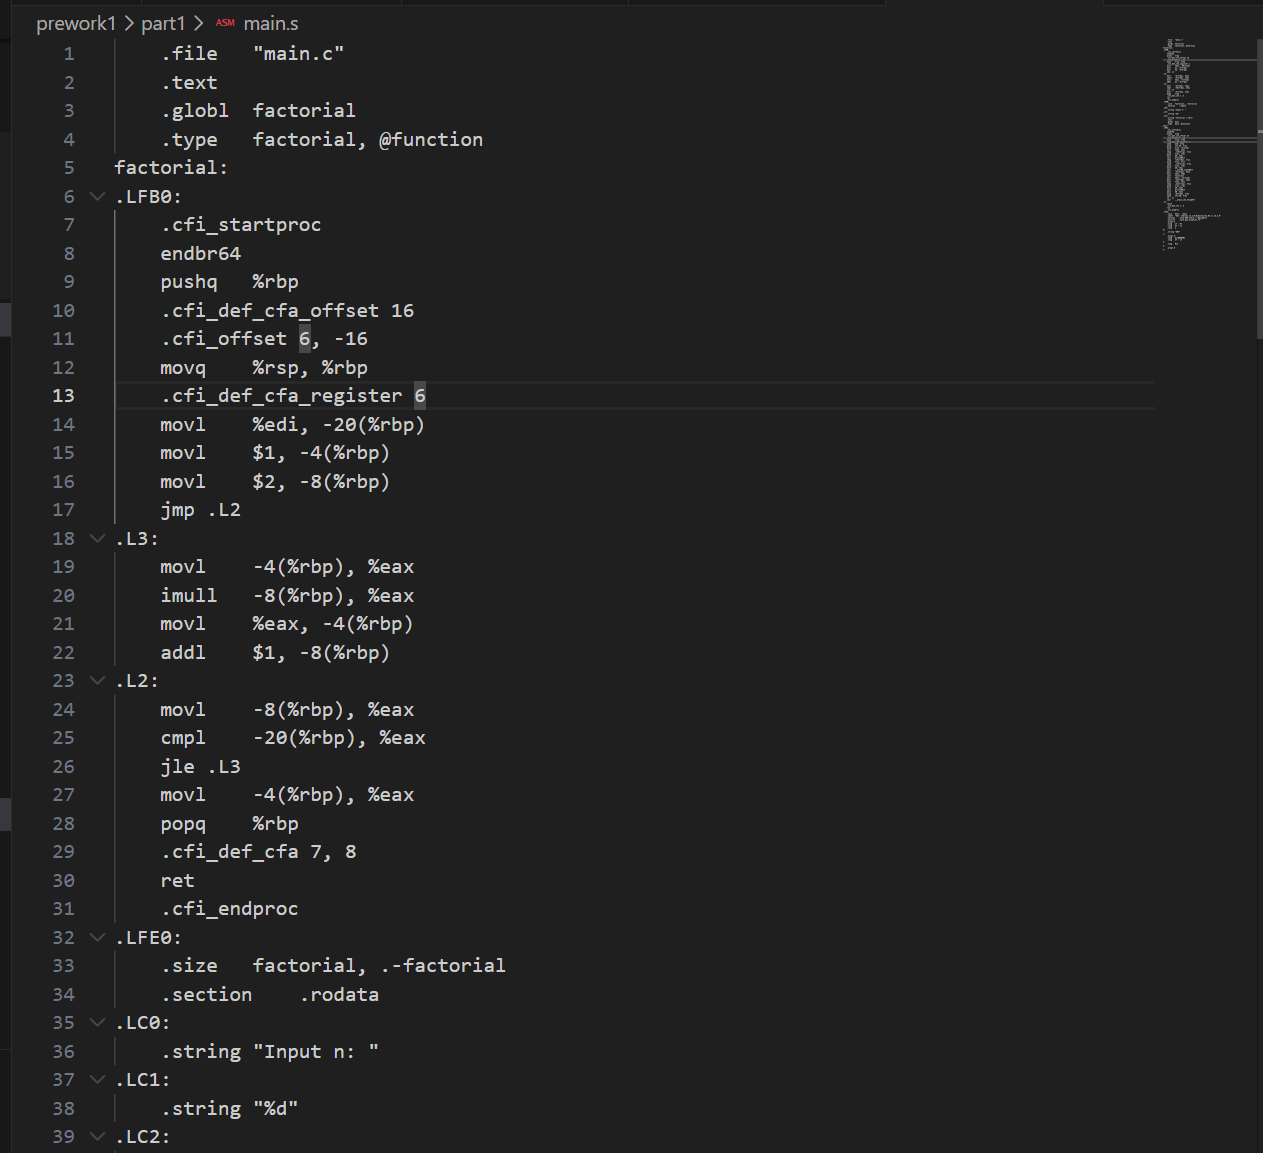
\includegraphics[width=\textwidth]
{images/part1/part1_assembly.png}
\caption{x86-64 汇编}
\end{subfigure}

\caption{LLVM IR 与目标汇编代码}
\label{fig:ir-asm}
\end{figure}

LLVM IR 已经明显低于 C 语言的抽象层次，但仍不依赖具体机器寄存器。继续生成 x86-64 汇编后，局部变量开始表现为寄存器或者栈偏移，条件和循环进一步转换为比较与跳转指令。

目标文件阶段通过 \texttt{nm} 可以观察到 \texttt{factorial} 和 \texttt{main} 已在当前翻译单元中定义，而 \texttt{printf}、\texttt{scanf} 等符号仍需要外部库提供。经过链接后，最终形成 ELF 可执行文件。

\begin{figure}[H]
\centering
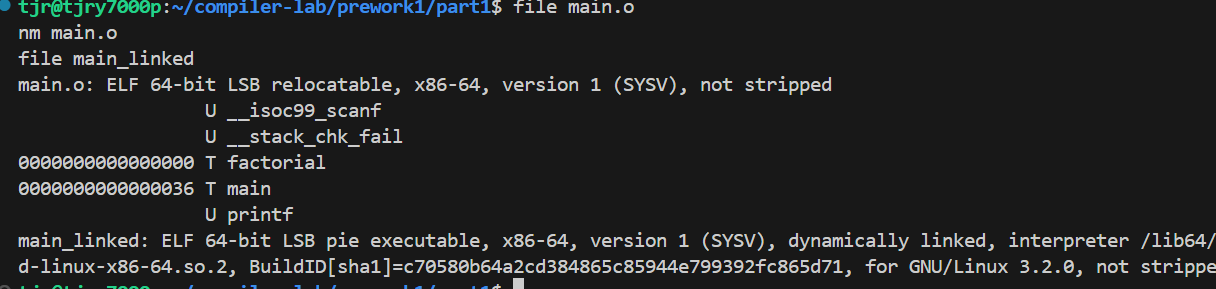
\includegraphics[width=0.78\textwidth]
{images/part1/part1_object_link.png}
\caption{目标文件符号与链接结果}
\label{fig:object-link}
\end{figure}

这一现象说明，“编译完成”和“程序已经可以独立执行”并不是同一个概念。编译器可以先生成包含未解析外部符号的目标文件，再由链接器负责将目标文件和所需库组合起来。

\subsection{优化前后的代码差异}

实验还分别生成了 \texttt{-O0} 与 \texttt{-O2} 版本的汇编代码。未优化情况下，\texttt{i} 和 \texttt{result} 等局部变量频繁通过栈访问，控制流也基本保持源程序的形式。

例如 \texttt{-O0} 中循环主体包含：

\begin{lstlisting}
movl    -4(%rbp), %eax
imull   -8(%rbp), %eax
movl    %eax, -4(%rbp)
addl    $1, -8(%rbp)
\end{lstlisting}

而 \texttt{-O2} 中对应循环被重新组织为：

\begin{lstlisting}
imull   %eax, %edx
leal    1(%rax), %ecx
addl    $2, %eax
imull   %ecx, %edx
\end{lstlisting}

可以看到优化后更多中间值直接保存在寄存器中，而且一次循环可以完成两个相邻乘数的累乘，减少循环控制次数。

此外，\texttt{-O2} 版本的 \texttt{main} 中原有的 \texttt{call factorial} 消失，阶乘计算逻辑被直接展开到调用位置，体现出函数内联优化。

因此，编译器优化的本质并不是简单缩短汇编文件，而是在保证程序外部可观察语义不变的前提下重新组织数据流、控制流和函数调用，从而降低访存、分支和调用等开销。

% =========================================================
\section{SysY 程序设计与两种目标表示}
% =========================================================

\subsection{SysY 测试程序设计}

第二部分需要手工完成 LLVM IR 与 RISC-V 汇编，因此测试程序既不能过于简单，也不宜包含大量重复结构。本实验设计的 SysY 程序使用 \texttt{calc(int n)} 函数作为主要计算过程，并在主函数中完成输入、边界处理和最终结果输出。

程序首先调用 \texttt{getint()} 读取整数 $n$。为了保证数组访问安全，将 $n$ 限制在 $[1,8]$ 范围内。随后 \texttt{calc} 函数执行循环：当 $i+1$ 为偶数时，将其平方写入 \texttt{values[i]}；否则写入其相反数，并将数组元素逐项累加。

例如，当

\[
n=5
\]

时，数组前五项为：

\[
[-1,\ 4,\ -3,\ 16,\ -5],
\]

因此

\[
\texttt{calc}(5)
=
-1+4-3+16-5
=
11.
\]

主函数还会计算：

\[
5/2=2,
\qquad
5\bmod 2=1,
\]

并加入常量 \texttt{BASE=3}，因此最终结果为：

\[
11+2+1+3=17.
\]

这一结果也可以作为后续 LLVM IR 和 RISC-V 两种实现是否保持语义一致的测试基准。

程序覆盖的主要语言结构如下。

\begin{table}[H]
\centering
\caption{SysY 测试程序覆盖的语言特性}
\begin{tabularx}{\textwidth}{@{}p{3.2cm}X@{}}
\toprule
类别 & 使用内容 \\
\midrule

数据定义 &
常量、局部变量、一维整型数组 \\

数值运算 &
加、减、乘、除、取模、一元负号 \\

控制结构 &
嵌套 \texttt{if/else}、\texttt{while} \\

函数 &
用户函数、参数、返回值、函数调用 \\

运行时接口 &
\texttt{getint}、\texttt{putint}、\texttt{putch} \\

\bottomrule
\end{tabularx}
\end{table}

这种设计使程序规模保持适中，同时能够在低层实现中观察数组寻址、基本块跳转、循环、函数调用、参数传递和整数运算等关键机制。

\subsection{LLVM IR 实现}

\noindent
\textbf{主要负责人：王帅（2413995）}

\wsplaceholder{
建议补充约 1 页左右。首先说明 \texttt{calc} 和 \texttt{main}
的基本块划分；再说明数组通过 \texttt{alloca} 和
\texttt{getelementptr} 完成地址计算，条件和循环通过
\texttt{icmp/br} 实现；最后说明 \texttt{getint}、
\texttt{putint} 和 \texttt{putch} 的声明、运行时库链接方式及测试结果。
正文建议放 1 张关键 LLVM IR 截图和 1 张最终测试截图，不粘贴完整 main.ll。
}

% =========================================================
\section{RISC-V 汇编实现与验证}
% =========================================================

\subsection{运行环境与总体实现}

\noindent
\textbf{主要负责人：谭锦睿（2412771）}

RISC-V 部分采用 RV64 汇编手工实现上述 SysY 程序。由于实验机本身为 x86-64 环境，因此程序使用 RISC-V 交叉工具链生成目标文件，再通过 qemu-riscv64 执行。

正式实现前，首先编写只调用 \texttt{putint} 和 \texttt{putch} 的最小汇编程序，并与 \texttt{libsysy\_riscv.a} 链接。程序能够正确输出 123，说明交叉编译器、SysY RISC-V 运行时库以及 QEMU 已经能够形成完整执行链路。

\begin{figure}[H]
\centering
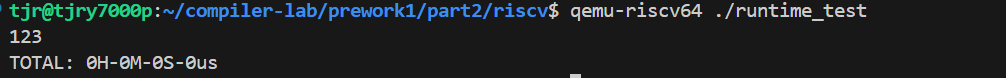
\includegraphics[width=0.72\textwidth]
{images/riscv/riscv_runtime_test.png}
\caption{SysY RISC-V 运行时库验证}
\label{fig:riscv-runtime}
\end{figure}

随后实现完整的 \texttt{calc} 和 \texttt{main}。主要需要解决四个问题：局部变量如何保存、数组下标如何转换为实际地址、高级语言控制结构如何变成分支与跳转，以及函数参数和返回值如何在寄存器之间传递。

\subsection{栈帧与数组寻址}

\texttt{calc} 函数包含 \texttt{values[8]}、\texttt{i}、\texttt{result} 以及参数 \texttt{n}。一个 SysY \texttt{int} 占 4 字节，因此数组本身需要 32 字节。实现中统一为该函数分配 48 字节栈帧。

\begin{table}[H]
\centering
\caption{\texttt{calc} 函数主要栈空间布局}
\begin{tabular}{ll}
\toprule
位置 & 内容 \\
\midrule
\texttt{0(sp)--28(sp)} & \texttt{values[0]--values[7]} \\
\texttt{32(sp)} & \texttt{i} \\
\texttt{36(sp)} & \texttt{result} \\
\texttt{40(sp)} & 参数 \texttt{n} \\
\bottomrule
\end{tabular}
\end{table}

48 字节本身是 16 的整数倍，因此调用过程中能够保持栈对齐。

对于数组元素

\[
\texttt{values}[i],
\]

由于每个元素宽度为 4 字节，因此其地址满足：

\[
\mathrm{addr}(\texttt{values}[i])
=
\mathrm{sp}+4i.
\]

汇编中可以先通过左移两位得到 $4i$：

\[
i \ll 2 = 4i,
\]

再与 \texttt{sp} 相加得到数组元素地址。

这个过程体现出高级语言中的数组下标访问，在机器层实际上需要转换为“基地址 + 偏移量”的地址计算。

\subsection{控制流与整数运算}

源程序中的：

\[
\texttt{while}(i<n)
\]

在汇编中不再存在一个独立的“循环”指令，而是转换为比较和跳转。

每轮循环开始时先比较 $i$ 与 $n$。如果

\[
i\ge n,
\]

则跳转到循环结束标签；否则继续执行循环体。循环体结束后再无条件跳回条件判断位置。

同样，源程序中的：

\[
(i+1)\bmod2==0
\]

使用 \texttt{remw} 计算余数，再根据结果是否为 0 跳转到不同分支。因此，从目标代码角度看，\texttt{while}、\texttt{if} 和 \texttt{else} 最终都可以归结为基本块之间的控制流转移。

虽然目标体系结构为 RV64，但 SysY 中的 \texttt{int} 为 32 位整数。因此本程序主要使用：

\begin{center}
\texttt{addw}、
\texttt{addiw}、
\texttt{subw}、
\texttt{mulw}、
\texttt{divw}、
\texttt{remw}
\end{center}

等 32 位整数运算指令，使目标代码的整数语义与 SysY 保持一致。

\subsection{函数调用与运行时库}

RISC-V 调用约定规定整数参数和返回值优先通过 \texttt{a0--a7} 等参数寄存器进行传递。

本程序调用：

\[
\texttt{calc}(n)
\]

之前，首先将参数 $n$ 放入 \texttt{a0}；函数结束后，返回结果同样通过 \texttt{a0} 返回。

\texttt{main} 还需要调用：

\[
\texttt{getint},
\qquad
\texttt{putint},
\qquad
\texttt{putch}.
\]

这些函数由 SysY 运行时库提供。

由于执行 \texttt{call} 会覆盖返回地址寄存器 \texttt{ra}，因此 \texttt{main} 在函数入口处先将 \texttt{ra} 保存到栈中，结束前再恢复。

这一实现说明，高级语言中的一次函数调用，在目标代码层面实际上还需要处理参数位置、返回值、返回地址和栈空间恢复等问题。

\subsection{汇编、链接与执行验证}

首先将汇编文件生成可重定位目标文件：

\begin{lstlisting}
riscv64-unknown-elf-gcc main.s -c -o main.o -w
\end{lstlisting}

然后与 SysY RISC-V 运行时库进行静态链接：

\begin{lstlisting}
riscv64-unknown-elf-gcc main.o -o main \
  -L../lib -lsysy_riscv -static -mcmodel=medany \
  -Wl,--no-relax,-Ttext=0x90000000
\end{lstlisting}

其中 \texttt{-L../lib} 指定运行时库目录，\texttt{-lsysy\_riscv} 链接课程提供的 RISC-V SysY 运行时库，\texttt{-static} 表示使用静态链接。

生成结果如图~\ref{fig:riscv-build} 所示。可以看到，\texttt{main.o} 为 RISC-V 可重定位目标文件，而最终的 \texttt{main} 已经是静态链接的 64 位 RISC-V ELF 可执行程序。

\begin{figure}[H]
\centering
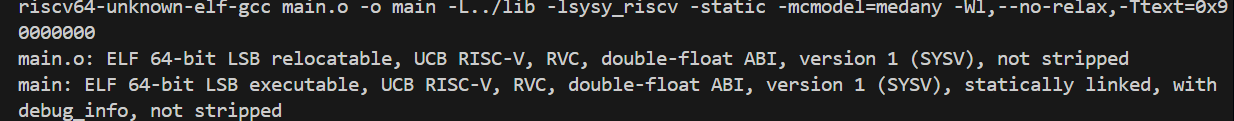
\includegraphics[width=0.80\textwidth]
{images/riscv/riscv_build.png}
\caption{RISC-V 汇编与链接结果}
\label{fig:riscv-build}
\end{figure}

验证阶段选取 0、1、4、5、8 和 10 六组输入。除了普通输入外，0 和 10 专门用于检查源程序中的上下界修正逻辑。

\begin{table}[H]
\centering
\caption{RISC-V 程序测试结果}
\begin{tabular}{ccccc}
\toprule
输入 & 实际参与计算的 $n$ & 预期结果 & RISC-V 输出 & 验证 \\
\midrule
0  & 1 & 3   & 3   & 正确 \\
1  & 1 & 3   & 3   & 正确 \\
4  & 4 & 21  & 21  & 正确 \\
5  & 5 & 17  & 17  & 正确 \\
8  & 8 & 111 & 111 & 正确 \\
10 & 8 & 111 & 111 & 正确 \\
\bottomrule
\end{tabular}
\end{table}

\begin{figure}[H]
\centering
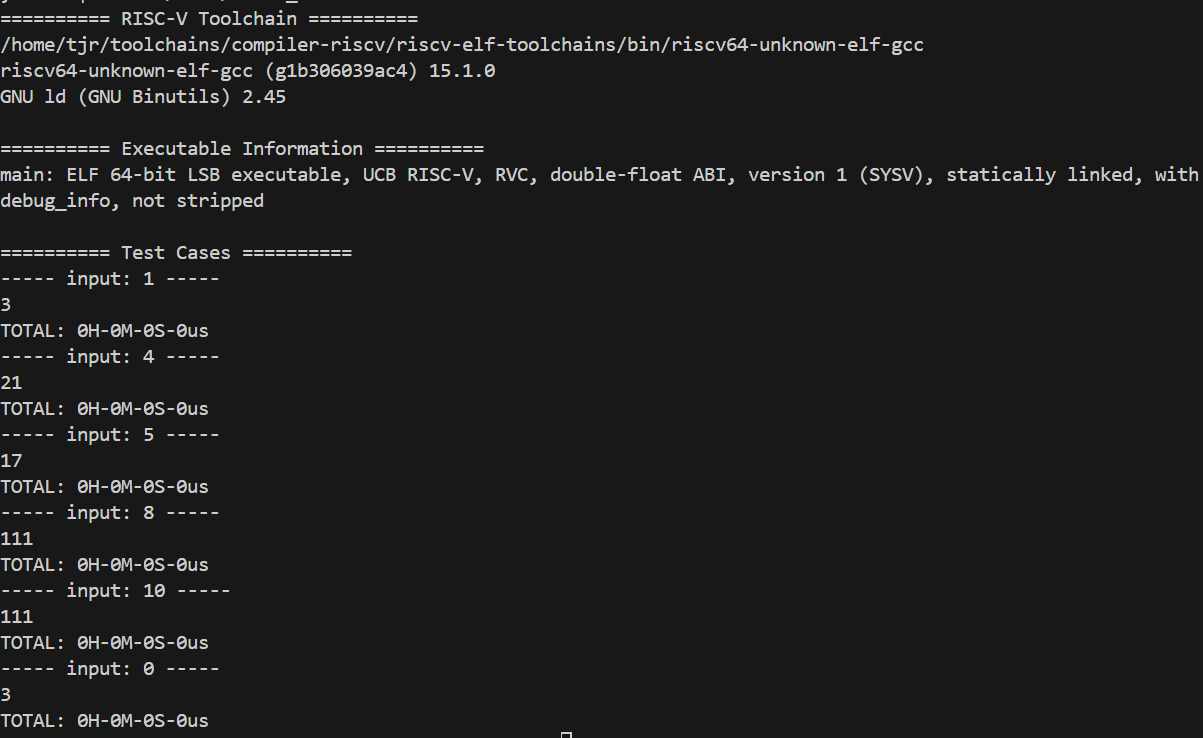
\includegraphics[width=0.84\textwidth]
{images/riscv/riscv_validation.png}
\caption{RISC-V 多组输入执行结果}
\label{fig:riscv-validation}
\end{figure}

六组测试全部得到预期结果。输入 0 被修正为 1，输入 10 被限制为 8，说明上下界条件分支正确；其余输入的结果同时验证了循环、数组地址计算、乘除取模、函数调用以及运行时输出等实现。

因此，可以确认手写 RISC-V 程序在这些测试输入下与原 SysY 程序保持一致的可观察行为。

% =========================================================
\section{LLVM IR 与 RISC-V 实现结果比较}
% =========================================================

\wsplaceholder{
王帅完成 LLVM IR 后，在此加入一个简短结果表即可。
建议仍使用输入 0、1、4、5、8、10，
表格包含“输入、预期结果、LLVM IR 输出、RISC-V 输出”四列。
如果结果全部一致，再用一段话说明两种低层实现均保持了相同的 SysY 源程序语义。
}

% 示例：
%
% \begin{table}[H]
% \centering
% \caption{LLVM IR 与 RISC-V 执行结果比较}
% \begin{tabular}{cccc}
% \toprule
% 输入 & 预期结果 & LLVM IR & RISC-V \\
% \midrule
% 0  & 3   & 3   & 3 \\
% 1  & 3   & 3   & 3 \\
% 4  & 21  & 21  & 21 \\
% 5  & 17  & 17  & 17 \\
% 8  & 111 & 111 & 111 \\
% 10 & 111 & 111 & 111 \\
% \bottomrule
% \end{tabular}
% \end{table}

% =========================================================
\section{进阶探索：MLIR 与 AscendNPU IR}
% =========================================================

\subsection{从 LLVM IR 到多层中间表示}

基础实验中的 LLVM IR 提供了一种较统一的中间表示。C 程序被转换为 \texttt{alloca}、\texttt{load}、\texttt{store}、\texttt{icmp}、\texttt{br} 等较低层操作之后，源语言中的大部分高级结构已经被消除。这种设计有利于为不同前端和不同目标机器建立统一接口。

但面向 AI 加速器时，程序通常还包含张量、向量运算、专用存储空间和数据搬运等更丰富的语义。如果过早全部下降到统一低层指令，这些信息可能难以继续用于针对硬件特点的优化。

MLIR，即 Multi-Level Intermediate Representation，采用多层中间表示思想，通过 Dialect 描述不同抽象层次的操作。编译过程可以先保留较高层领域语义，再经过多个 Pass 逐步下降：

\[
\text{High-level IR}
\rightarrow
\text{Domain Dialect}
\rightarrow
\text{Hardware Dialect}
\rightarrow
\text{Low-level IR}.
\]

因此，lowering 不再只是“一次从高级语言变成低层 IR”，而可以理解为多个中间表示之间连续降低抽象层次的过程。

\subsection{AscendNPU IR 与 VecAdd}

题目提供的 AscendNPU IR VecAdd 示例展示了这一思想在昇腾 NPU 编译中的应用。

向量加法在数学上只是：

\[
C=A+B,
\]

但在实际设备上执行时，还需要考虑输入数据位于什么存储空间、何时搬入片上缓冲区、由什么计算单元完成向量运算，以及何时将结果写回。

因此，其核心数据流可以抽象为：

\[
\mathrm{GM}
\rightarrow
\mathrm{UB}
\rightarrow
\mathrm{Vector\ Add}
\rightarrow
\mathrm{GM}.
\]

其中 GM 表示较大的全局存储空间，UB 表示更靠近计算单元的片上缓冲空间。

相比普通 LLVM IR 中较通用的 \texttt{load/store}，这类专用 Dialect 可以在中间表示中显式保留存储层次、数据搬运以及向量运算等信息，从而使编译器能够围绕目标硬件特点执行更有针对性的优化。

结合 VecAdd 示例，可以将其 lowering 流程概括为：

\[
\text{通用 MLIR}
\rightarrow
\text{AscendNPU 专用 Dialect}
\rightarrow
\text{更低层硬件表示}
\rightarrow
\text{设备 Kernel}.
\]

\subsection{与 LLVM IR 的比较}

\begin{table}[H]
\centering
\caption{LLVM IR 与 MLIR/AscendNPU IR 的特点比较}
\begin{tabularx}{\textwidth}{@{}p{2.8cm}X X@{}}
\toprule
比较项 & LLVM IR & MLIR / AscendNPU IR \\
\midrule

抽象层次 &
以相对统一的低层表示为核心 &
允许多个不同抽象层次的 Dialect 共存 \\

扩展方式 &
围绕统一 IR 指令体系进行处理 &
可以面向领域和硬件定义专用 Dialect \\

硬件信息 &
通常在后端逐步体现 &
可以较早保留存储空间、数据搬运和向量操作 \\

优化方式 &
主要围绕 LLVM IR 和目标后端 &
可以在不同 Dialect 层分别执行针对性优化 \\

\bottomrule
\end{tabularx}
\end{table}

本实验使用普通 WSL2 环境，没有配置完整 CANN 和昇腾 NPU 设备，因此进阶部分主要采用官方示例阅读和 IR 静态分析的方式完成，没有将官方示例中的设备运行结果作为本机实验结果。

通过这一探索可以看出，现代 AI 编译器的中间端并不一定只依赖一种统一 IR，而可以在不同层次保留不同程度的语义信息，并通过渐进式 lowering 最终转换为目标硬件可以执行的代码。

% =========================================================
\section{总结}
% =========================================================

本实验围绕编译器从高级语言到目标程序的完整处理过程展开。第一部分通过 GCC 和 Clang/LLVM 的实际输出观察了预处理、词法分析、AST、LLVM IR、汇编、目标文件和链接等阶段，使课堂中较为抽象的编译流程与实际文件和指令建立了对应关系。

对 \texttt{-O0} 与 \texttt{-O2} 汇编代码的比较还表明，编译优化会重新组织寄存器使用、循环结构甚至函数调用方式，而不是简单地对源程序进行逐句翻译。优化的目标是在保持程序语义一致的前提下减少不必要的访存、分支和函数调用等开销。

第二部分选择同一个 SysY 程序作为语义基准，分别进行 LLVM IR 和 RISC-V 手工实现。RISC-V 部分进一步涉及局部变量的栈上布局、数组的基址加偏移寻址、条件和循环的跳转实现、RV64 环境中的 32 位整数运算以及函数调用约定。通过与 SysY 运行时库静态链接，并在 QEMU 中测试 0、1、4、5、8、10 六组输入，程序均得到与预期一致的结果。

进阶部分进一步从 LLVM IR 扩展到 MLIR 与 AscendNPU IR。VecAdd 示例表明，面向专用硬件时，中间表示不仅要描述“计算什么”，还可以显式保留“数据位于哪里、如何搬运以及由哪类计算单元处理”等信息。MLIR 通过多种 Dialect 和渐进式 lowering 为这种多层优化提供了更加灵活的基础。

通过本次实验，可以更加具体地认识到，编译器并不是一个简单的“源代码转机器码”工具，而是由多个层次的程序表示、转换、优化和运行时支持共同构成的系统。高级语言中的函数、变量、数组、循环和条件结构，最终都需要逐步落实为基本块、地址计算、寄存器、栈空间以及机器级控制流。

\end{document}